\begin{frame}{Intuition}
  \begin{itemize}[<+>]
    \item Managed runtimes use garbage collectors to abstract away manual memory management
    \item These languages are simple to program in (e.g. Python, Haskell) without malloc
    \item Under the hood objects are placed in heap pages that are managed by the OS paging policy
  \end{itemize}

  \begin{block}{Why might we disagree with the OS policy?}
    \begin{itemize}[<+>]
      \item MLP: memory level parallelism
      \item OS has no idea what's on our pages. Could be a linked list (low MLP); could be a \texttt{std::array} (high MLP)
      \item In fact, the OS does not care.
      \item Pointer chasing is expensive in low MLP objects. Latency is more affordable in high MLP objects
      \item Can we place our objects elsewhere? Where?
    \end{itemize}
  \end{block}
\end{frame}

\begin{frame}{Intuition}
  \begin{block}{Introduce: far memory}
    \begin{itemize}[<+>]
      \item Far memory is shared memory between devices that is cheaper and slower than RAM but faster than swap
      \item In HPC, we may accept the performance tradeoff if it means swapping fewer pages - overall still faster
      \item Thus, maybe some objects can live in near memory, others in far memory
      \item How can we automagically choose where heap objects live?
    \end{itemize}
  \end{block}
\end{frame}

\begin{frame}{Two Hurdles to Programming a GC}
  \begin{block}{What's the promotion policy?}
    \begin{itemize}[<+>]
      \item Deciding heuristics is incredibly difficult
      \item Entire papers come out of finding a single good heuristic
      \item Implementing somewhat hardware-based policies in software-level runtime also creates tension
    \end{itemize}
  \end{block}
  \begin{block}{How do I express that policy in code?}
    \begin{itemize}[<+>]
      \item Best case scenario imagine I'm a genius and come up with a perfect heuristic
      \item How in the world do I implement it?
      \item Do I recompile the entire runtime? That's horribly burdensome both on time and compute
      \item Do I write a custom GC policy? That's not as comparable to existing work
    \end{itemize}
  \end{block}
  \begin{block}{How do we add a dual heap to a production GC?}
    \begin{itemize}[<+>]
      \item Use \texttt{mmap} lol
    \end{itemize}
  \end{block}
\end{frame}

\begin{frame}{Our Contribution}
  Three core pillars of this presentation
  \begin{block}{Far Memory Support}
    \begin{itemize}[<+>]
      \item \texttt{mmap}-ed a region of DAX-based far memory to emulate CXL hardware with reasonable latency and bandwidth tradeoffs compared to DRAM.
    \end{itemize}
  \end{block}
  \begin{block}{Improved Programmability}
    A researcher could use this to implement smart(er) heuristics
    \begin{itemize}[<+>]
      \item Created an API that takes accessible runtime metadata about objects and calls a C function that returns where the object should be placed.
      \item Support first-class compiler attributes to hint whether object should go to far or near memory.
    \end{itemize}
  \end{block}
  \begin{block}{Low Overhead}
    \begin{itemize}[<+>]
      \item 20\% overhead of calling a custom policy over a default-supported one, by dynamically loading a shared object.
      \item In same ballpark as overhead of using Intel IPT
    \end{itemize}
  \end{block}
\end{frame}

\begin{frame}{Far memory support: the bandwidth/latency comparison are reasonable proxies for CXL}
  \begin{center}
    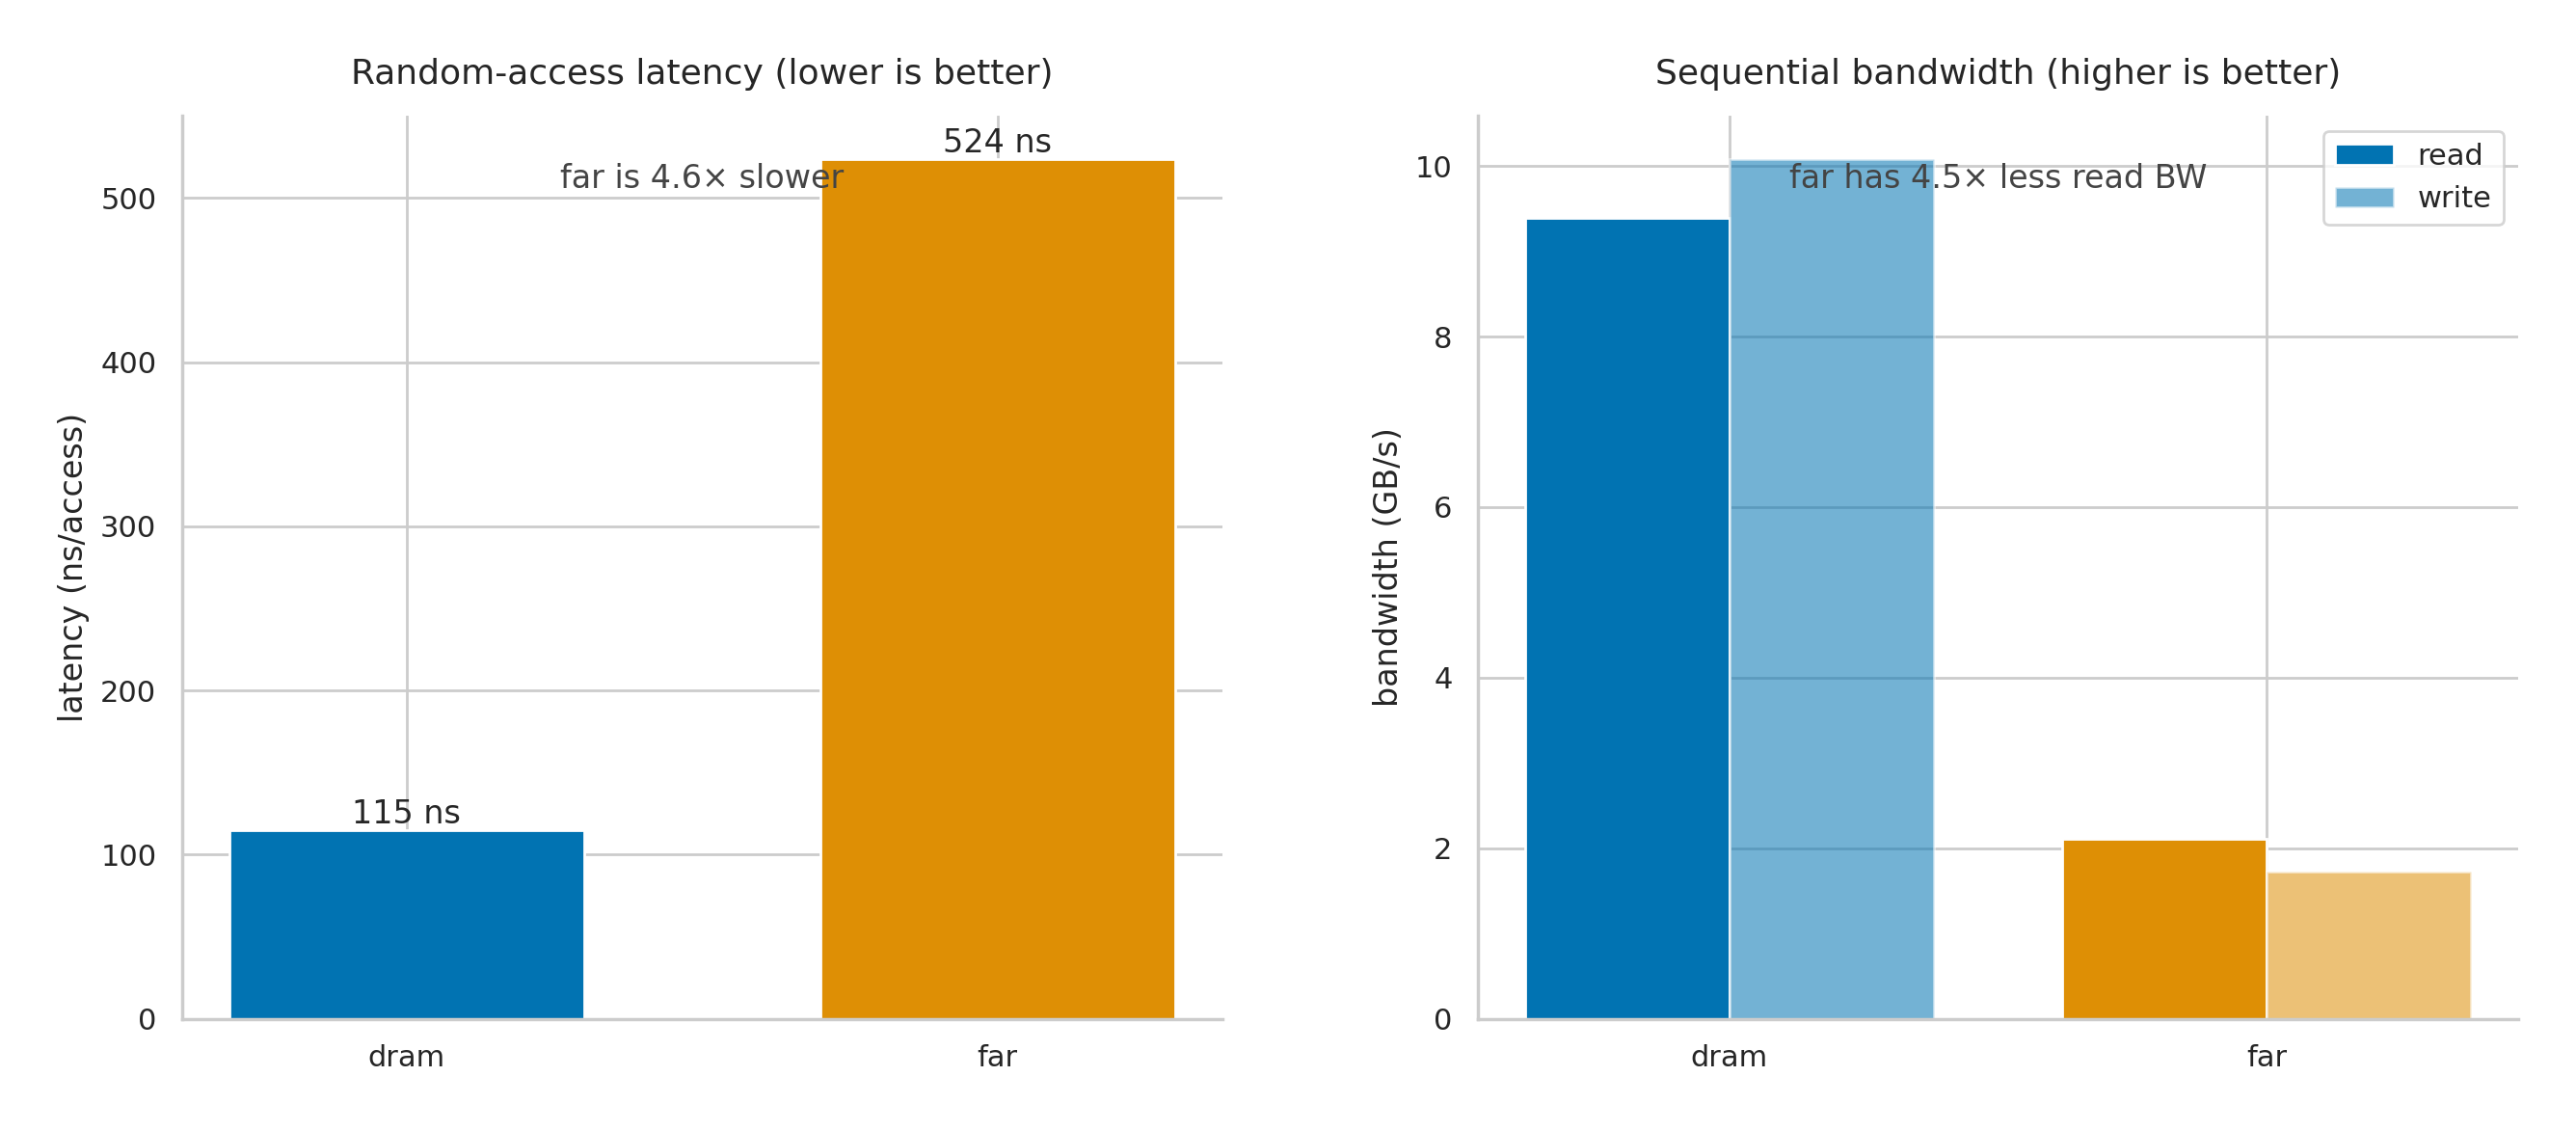
\includegraphics[width=\linewidth]{figures_new/fig3_hardware_comparison.png}
  \end{center}
\end{frame}

\begin{frame}{The GC can expose clean metadata to developers}
  \begin{center}
    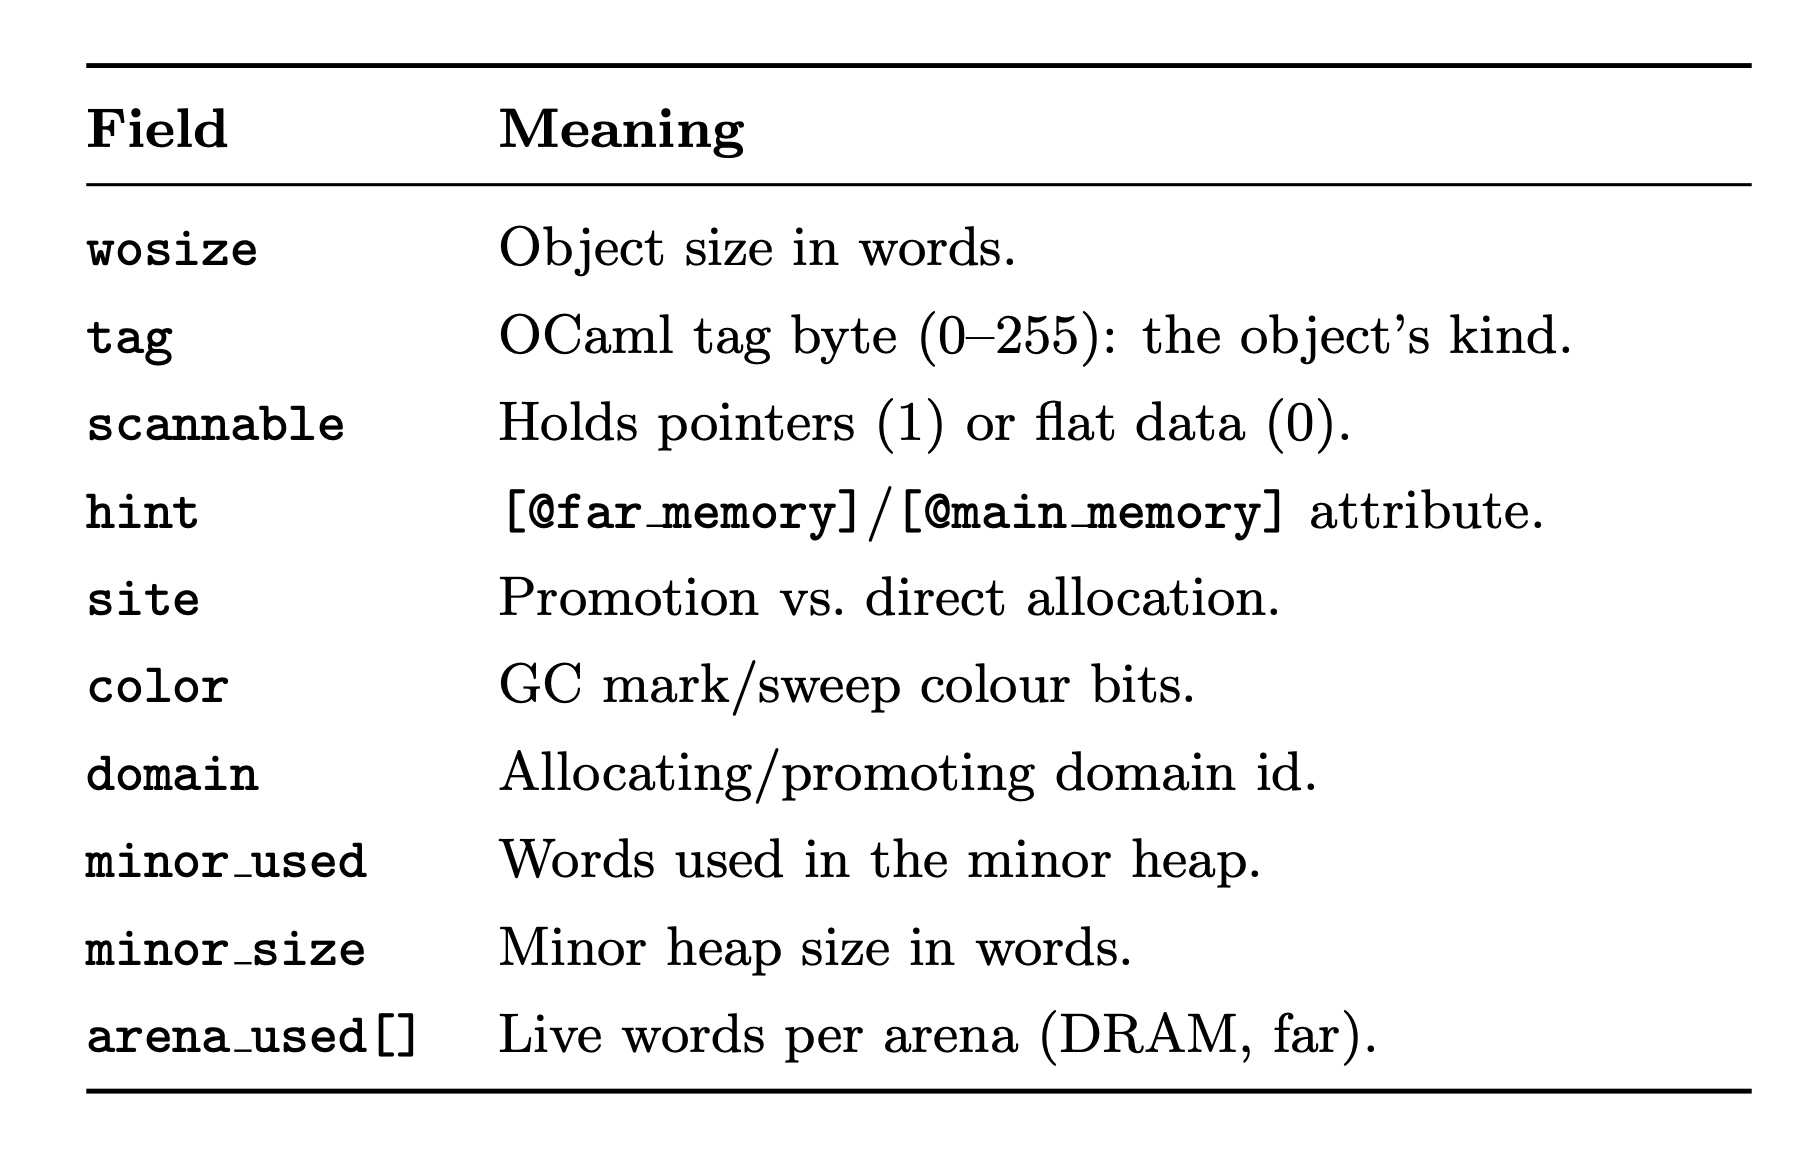
\includegraphics[width=\linewidth]{figures_new/fig0_fields.jpg}
  \end{center}
\end{frame}

\begin{frame}{That metadata is encoded as a simple, extensible struct in C}
  \begin{center}
    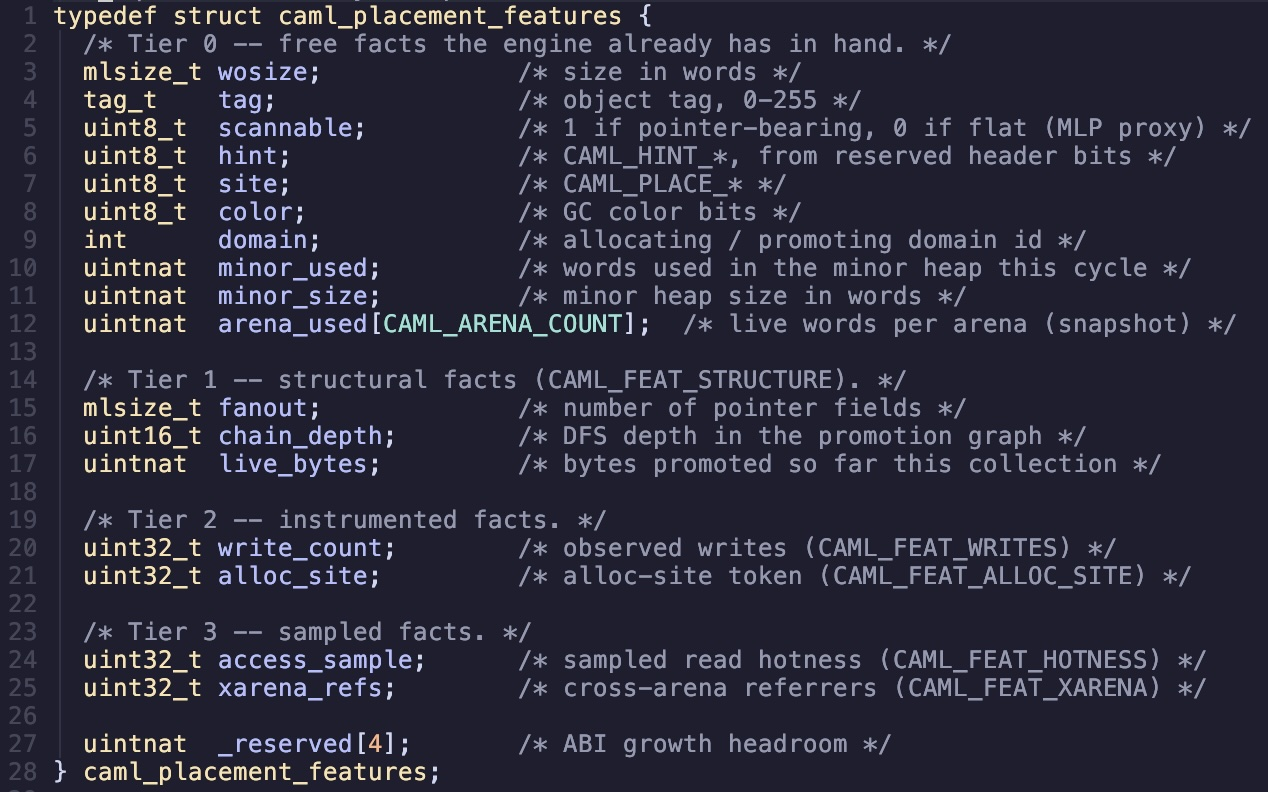
\includegraphics[width=\linewidth]{figures_new/fig6_placement_features_typedef.jpg}
  \end{center}
\end{frame}

\begin{frame}{Compiler attributes can be used to hint placement to far vs near memory}
  \begin{center}
    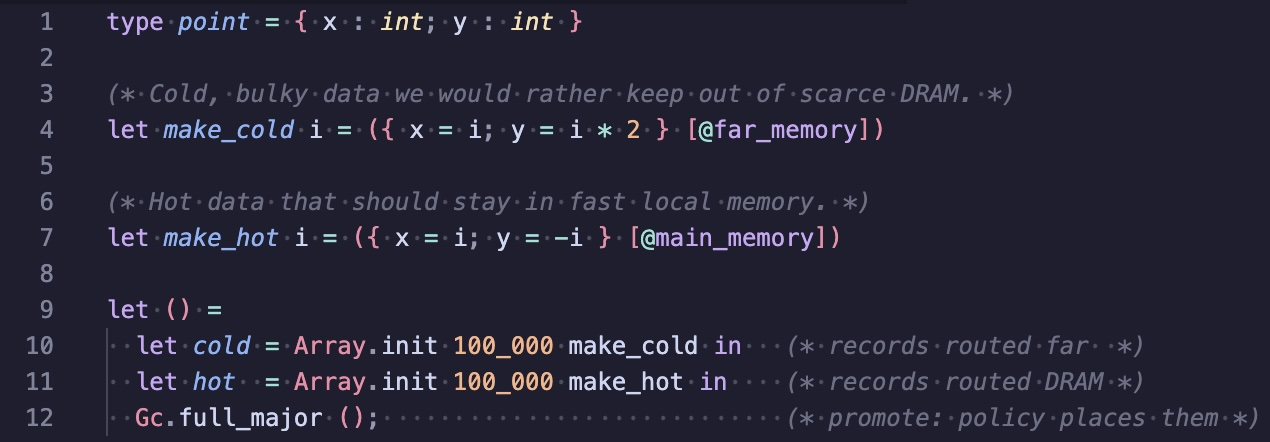
\includegraphics[width=\linewidth]{figures_new/fig4_ml_sample.jpg}
  \end{center}
\end{frame}

\begin{frame}{The metadata can be used to easily write custom policies in C}
  \begin{center}
    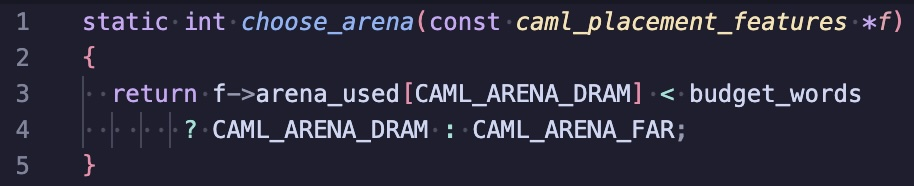
\includegraphics[width=0.5\linewidth]{figures_new/fig2b_trivial_policy.jpg}
    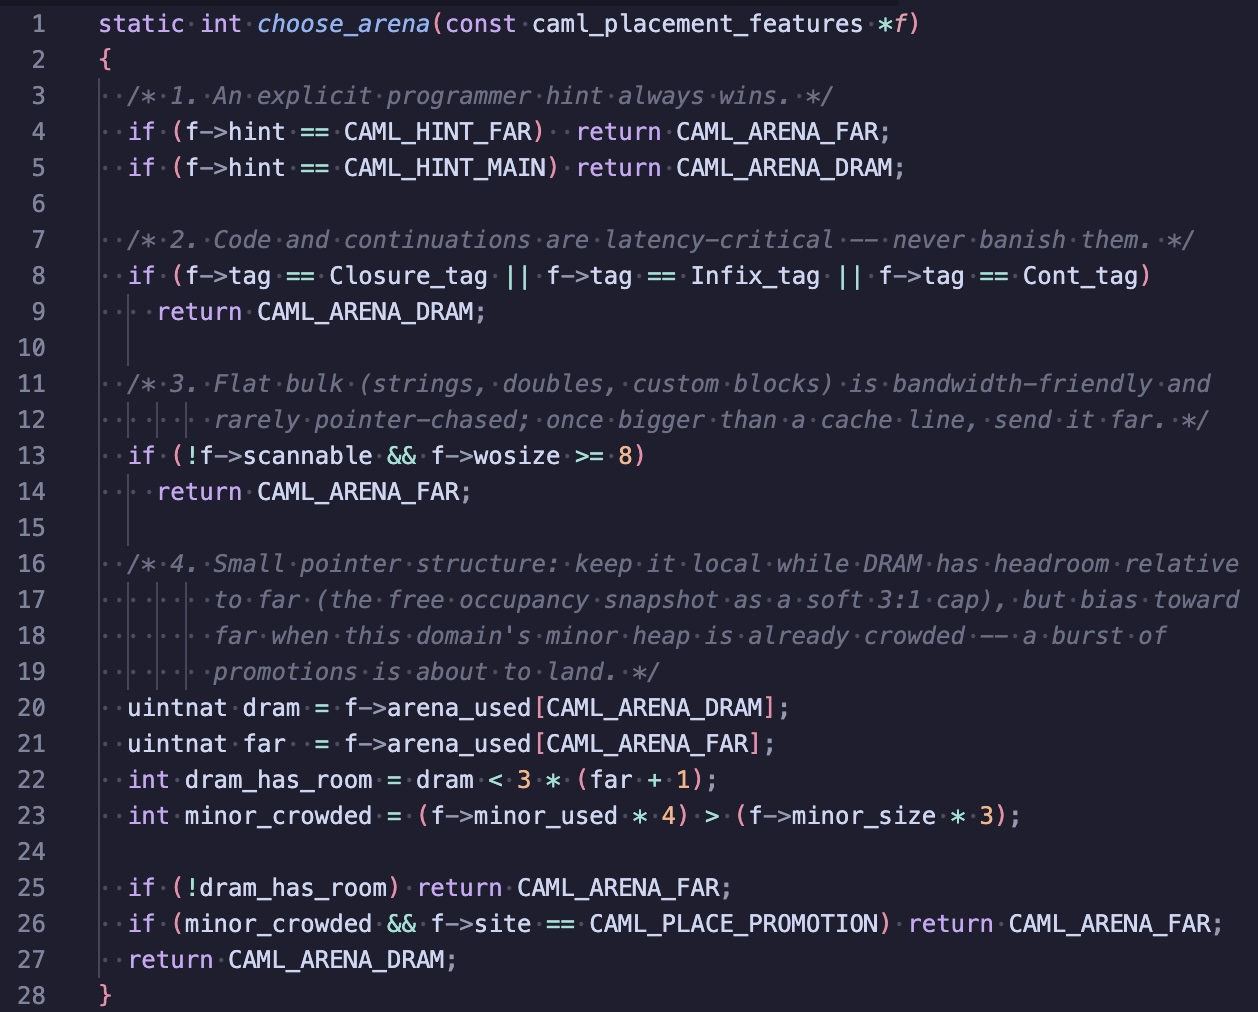
\includegraphics[width=0.5\linewidth]{figures_new/fig2a_complex_policy_still_simple.jpg}
  \end{center}
  Improved communication of policy between developers
\end{frame}

\begin{frame}{Policies make a measurable difference on low-MLP performance}
  \begin{center}
    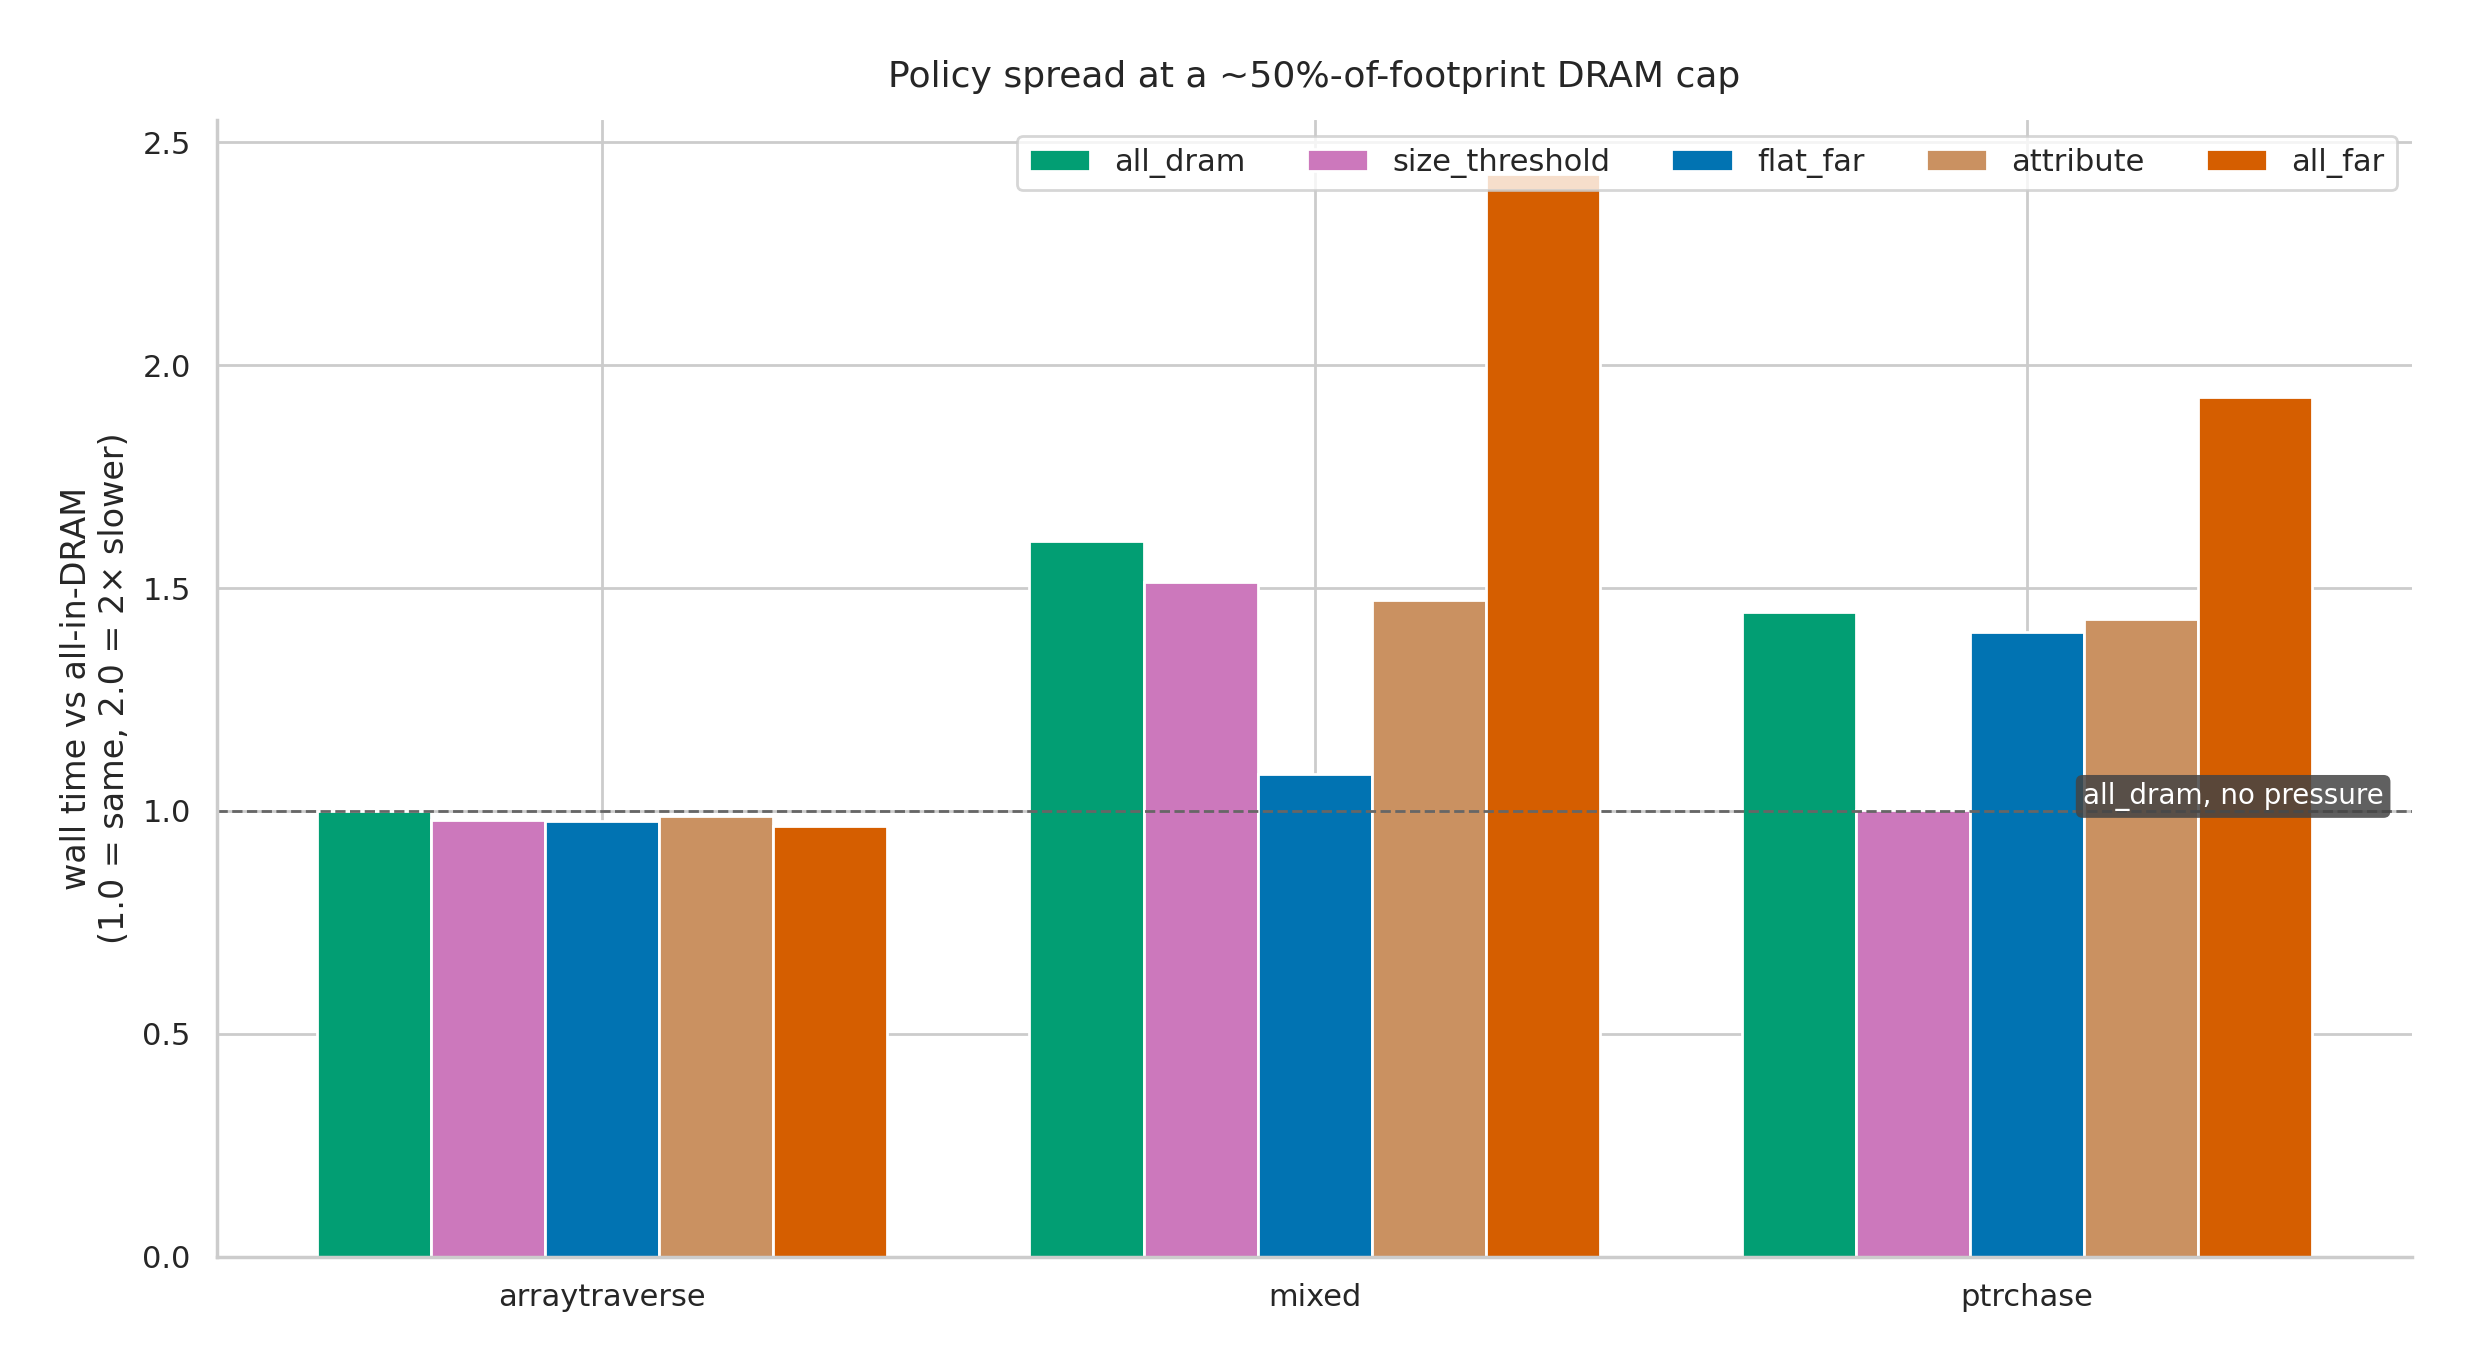
\includegraphics[width=\linewidth]{figures_new/fig1_policies_work.png}
  \end{center}
\end{frame}

\begin{frame}{The overhead of dynamically linking a \texttt{.so} is very low, upper bound 20\%}
  \begin{center}
    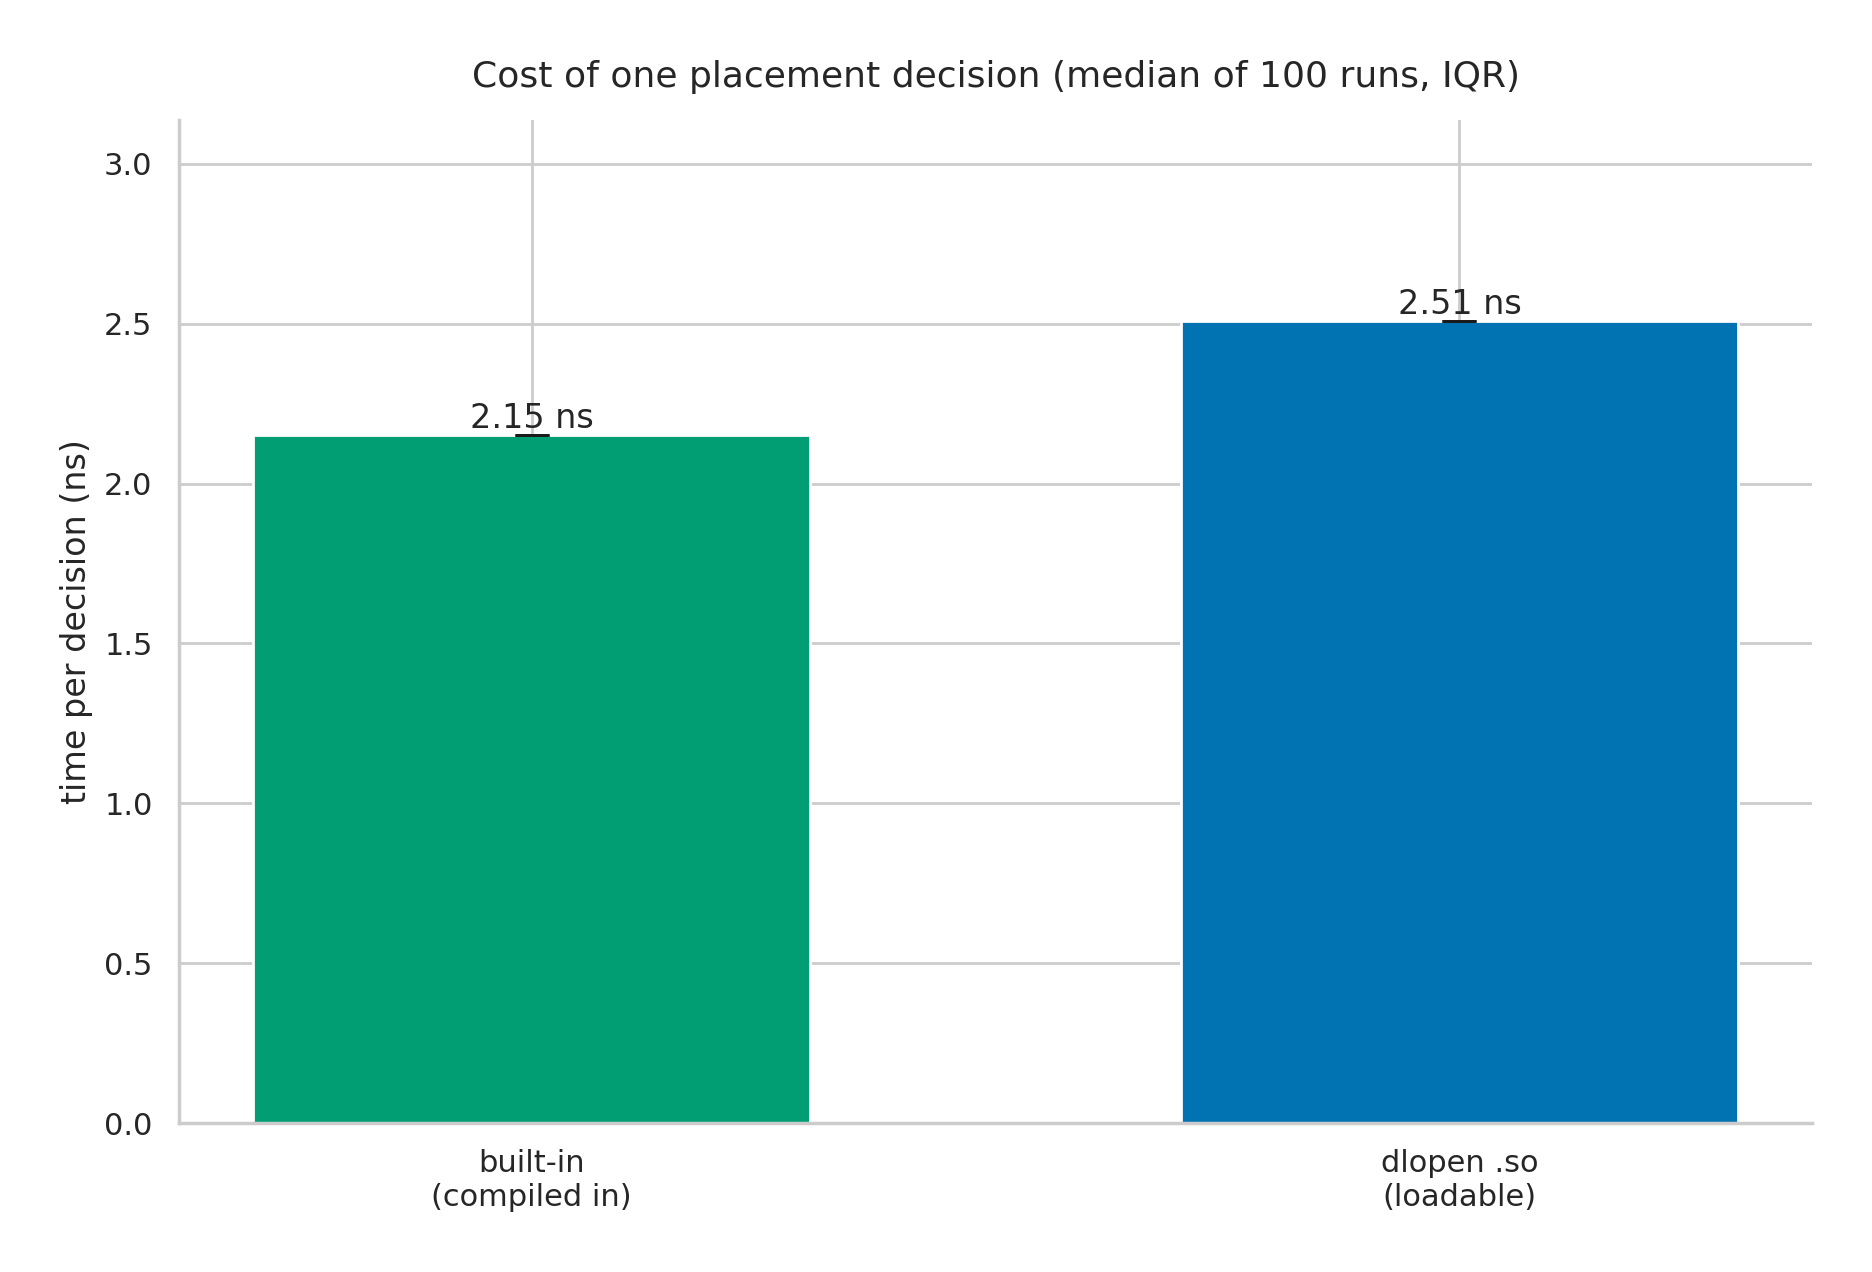
\includegraphics[width=0.8\linewidth]{figures_new/fig5_overhead.png}
  \end{center}
  Those black lines are error bars.
\end{frame}

\begin{frame}{Re: LLM Code Generation}
  We are all educators and probably care about reflecting on Claude usage
  \begin{itemize}[<+>]
    \item Consensus at work is to plan first for a long time (back and forth discussions) then give Claude free-reign
    \item The more specific, detailed, and impossible to misinterpret the prompt is, the better Claude's output becomes
    \item There is an art to talking with Claude in spoken English, which is a skill students can practice in classes
  \end{itemize}
  But all that requires me to
  \begin{itemize}[<+>]
    \item Understand the code Claude writes, which requires me to be able to write code by hand in the first place. So that honestly furthers the case for zero tolerance for AI-written code in 100 and 200 level courses, such that when someone gets to a 300 or 400 level, they \textit{can} responsibly autopilot with Claude and both get/understand reasonable output.
    \item Have a strong opinion on what Claude \textit{should} do and steer it in that direction. Those who use Claude because they don't know what to do vs those who use Claude because they know exactly what they want and how it should be automated achieve substantially different results.
  \end{itemize}
\end{frame}

\begin{frame}{Summary}
  \textbf{Problem:} Managed runtimes allocate heap objects without regard to memory topology, missing opportunities to exploit tiered (near/far) memory.

  \begin{block}{Our Contributions}
    \begin{itemize}[<+>]
      \item \textbf{Far memory support} - \texttt{mmap}-ed DAX region faithfully emulates CXL latency/bandwidth tradeoffs
      \item \textbf{Programmability} - GC exposes clean object metadata; custom placement policies are a single C function loaded as a \texttt{.so}; compiler attributes give first-class placement hints
      \item \textbf{Low overhead} - dynamic policy dispatch costs $\leq$20\%, on par with Intel IPT
    \end{itemize}
  \end{block}

  \begin{block}{Takeaways}
    \begin{itemize}[<+>]
      \item Placement policies can produce no gains at all or measurable gains; workload-dependent (as expected)
      \item Lowers the barrier for researchers to prototype and compare new heuristics without recompiling the runtime
      \item Enables code generation of policies, eases LLM-performed GC research
    \end{itemize}
  \end{block}
\end{frame}

\begin{frame}{Next Steps / Future Development}
  \begin{itemize}[<+>]
    \item Obviously write more heuristics/policies
    \item Encode ways to add hardware-based features to the metadata struct. Maybe we can use \texttt{perf} as a backend?
    \item Think about ways to move objects around depending on heuristic change over time. Existing work in PLab on handles can maybe be used here.
    \item Maybe we can give the GC a set of policies, and it can dynamically train a boosted tree on which features to favor. That would be resource intensive but could be an interesting proof of concept.
  \end{itemize}
\end{frame}
